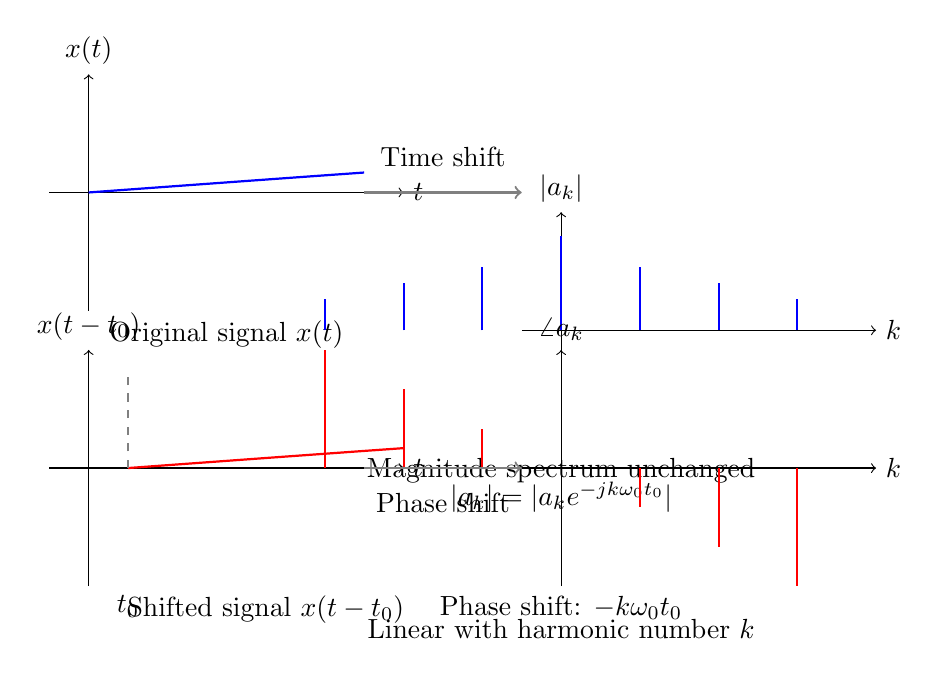
\begin{tikzpicture}
    % Time domain signal
    \begin{scope}[xshift=0cm, yshift=0cm]
        \draw[->] (-0.5,0) -- (4,0) node[right] {$t$};
        \draw[->] (0,-1.5) -- (0,1.5) node[above] {$x(t)$};
        \draw[thick, blue] plot[smooth, domain=0:3.5, samples=100] (\x, {sin(2*pi*\x/1.5)});
        \node[below] at (1.75,-1.5) {Original signal $x(t)$};
    \end{scope}
    
    % Shifted signal
    \begin{scope}[xshift=0cm, yshift=-3.5cm]
        \draw[->] (-0.5,0) -- (4,0) node[right] {$t$};
        \draw[->] (0,-1.5) -- (0,1.5) node[above] {$x(t-t_0)$};
        \draw[thick, red] plot[smooth, domain=0.5:4, samples=100] (\x, {sin(2*pi*(\x-0.5)/1.5)});
        \draw[dashed, gray] (0.5,0) -- (0.5,1.2);
        \node[below] at (0.5,-1.5) {$t_0$};
        \node[below] at (2.25,-1.5) {Shifted signal $x(t-t_0)$};
    \end{scope}
    
    % Frequency domain representation
    \begin{scope}[xshift=6cm, yshift=-1.75cm]
        \draw[->] (-0.5,0) -- (4,0) node[right] {$k$};
        \draw[->] (0,-1.5) -- (0,1.5) node[above] {$|a_k|$};
        
        % Original magnitude spectrum
        \draw[thick, blue] (0,0) -- (0,1.2);
        \draw[thick, blue] (1,0) -- (1,0.8);
        \draw[thick, blue] (2,0) -- (2,0.6);
        \draw[thick, blue] (3,0) -- (3,0.4);
        \draw[thick, blue] (-1,0) -- (-1,0.8);
        \draw[thick, blue] (-2,0) -- (-2,0.6);
        \draw[thick, blue] (-3,0) -- (-3,0.4);
        
        \node[below] at (0,-1.5) {Magnitude spectrum unchanged};
        \node[below] at (0,-1.8) {$|a_k| = |a_k e^{-jk\omega_0 t_0}|$};
    \end{scope}
    
    % Phase shift representation
    \begin{scope}[xshift=6cm, yshift=-3.5cm]
        \draw[->] (-0.5,0) -- (4,0) node[right] {$k$};
        \draw[->] (0,-1.5) -- (0,1.5) node[above] {$\angle a_k$};
        
        % Phase shift
        \draw[thick, red] (0,0) -- (0,0);
        \draw[thick, red] (1,0) -- (1,-0.5);
        \draw[thick, red] (2,0) -- (2,-1.0);
        \draw[thick, red] (3,0) -- (3,-1.5);
        \draw[thick, red] (-1,0) -- (-1,0.5);
        \draw[thick, red] (-2,0) -- (-2,1.0);
        \draw[thick, red] (-3,0) -- (-3,1.5);
        
        \node[below] at (0,-1.5) {Phase shift: $-k\omega_0 t_0$};
        \node[below] at (0,-1.8) {Linear with harmonic number $k$};
    \end{scope}
    
    % Arrows showing the relationship
    \draw[->, thick, gray] (3.5,0) -- (5.5,0);
    \draw[->, thick, gray] (3.5,-3.5) -- (5.5,-3.5);
    \node[above] at (4.5,0.2) {Time shift};
    \node[below] at (4.5,-3.7) {Phase shift};
\end{tikzpicture}
